\documentclass[../../Thesis.tex]{subfiles}
\begin{document}
\header{Research results}
\subheader{Ranking}
The graph XXX shows the ranking results for the different sets based on the title. Graph XXX displays the ranking results based on the abstract. Both graphs show both average and median ranks, based on the cosine-similarity between the article and journal embeddings or feature vectors.\\
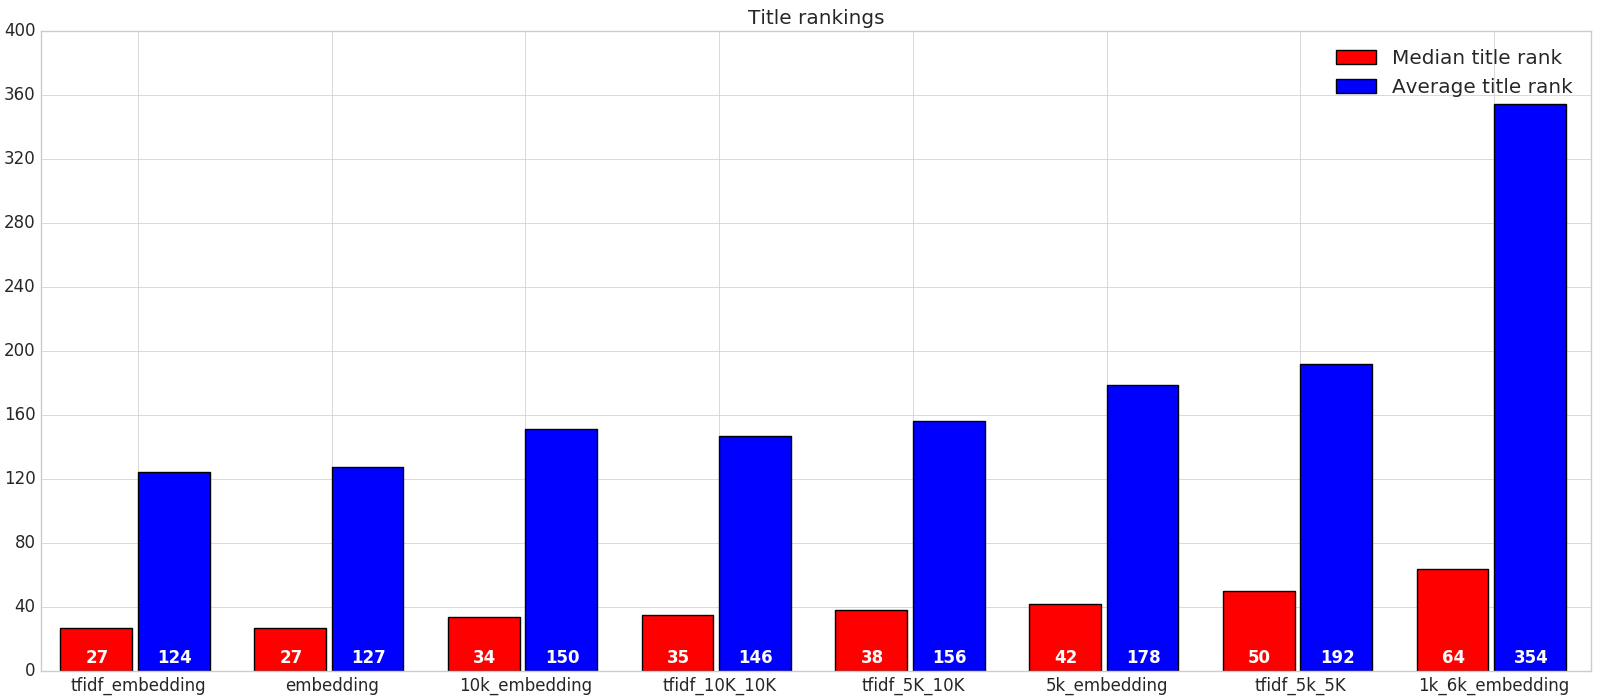
\includegraphics[width=6.5in]{Plots/Title_rankings}\\
\vspace{0.2in}\\
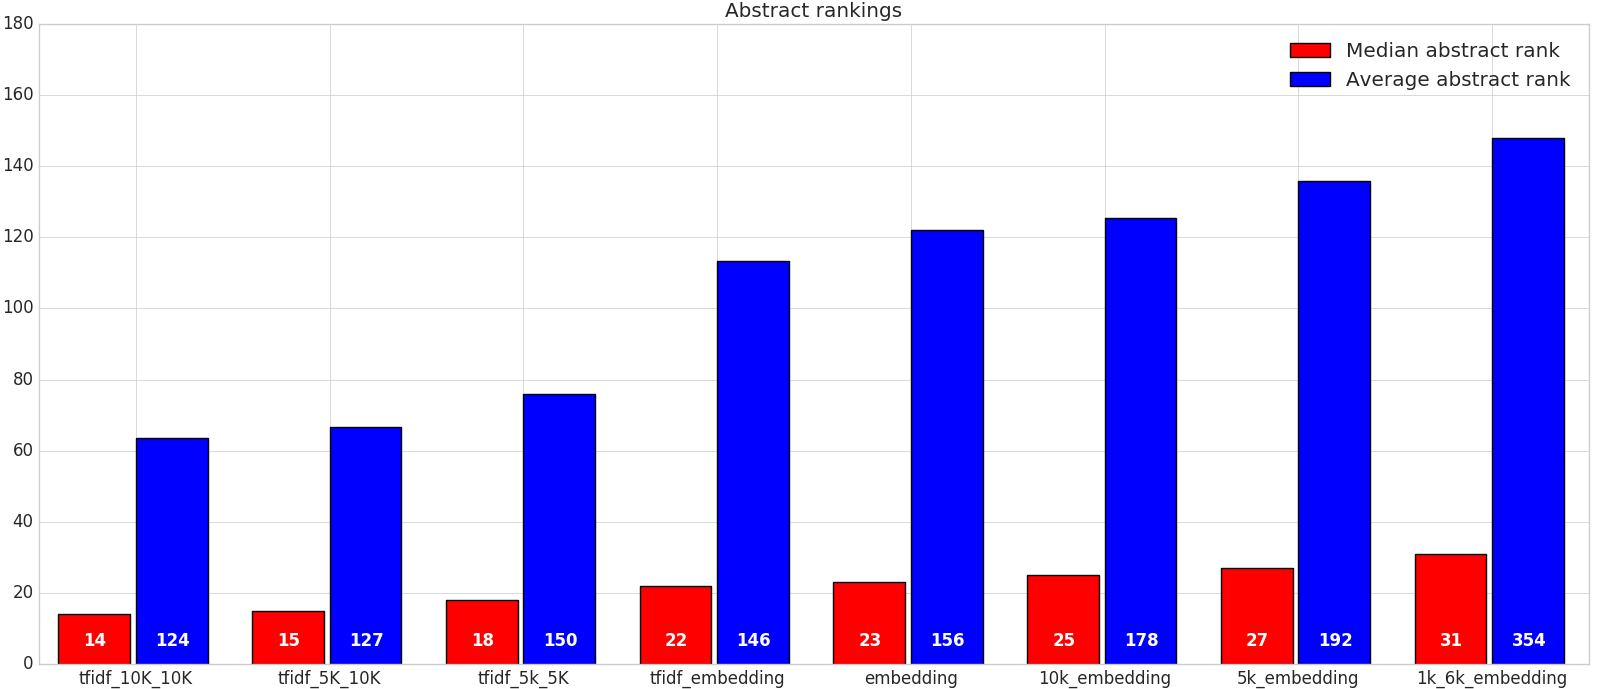
\includegraphics[width=6.5in]{Plots/Abstract_rankings}\\
\clearpage
\subheader{Rank distribution}
Graph XXX shows the rank distribution for the titles on, graph XXX shows this for the ranks based on the abstract. Both graphs use a logarithmic scale. These graphs give a detailled view of the ranks presented in the respective graphs XXX and XXX.\\
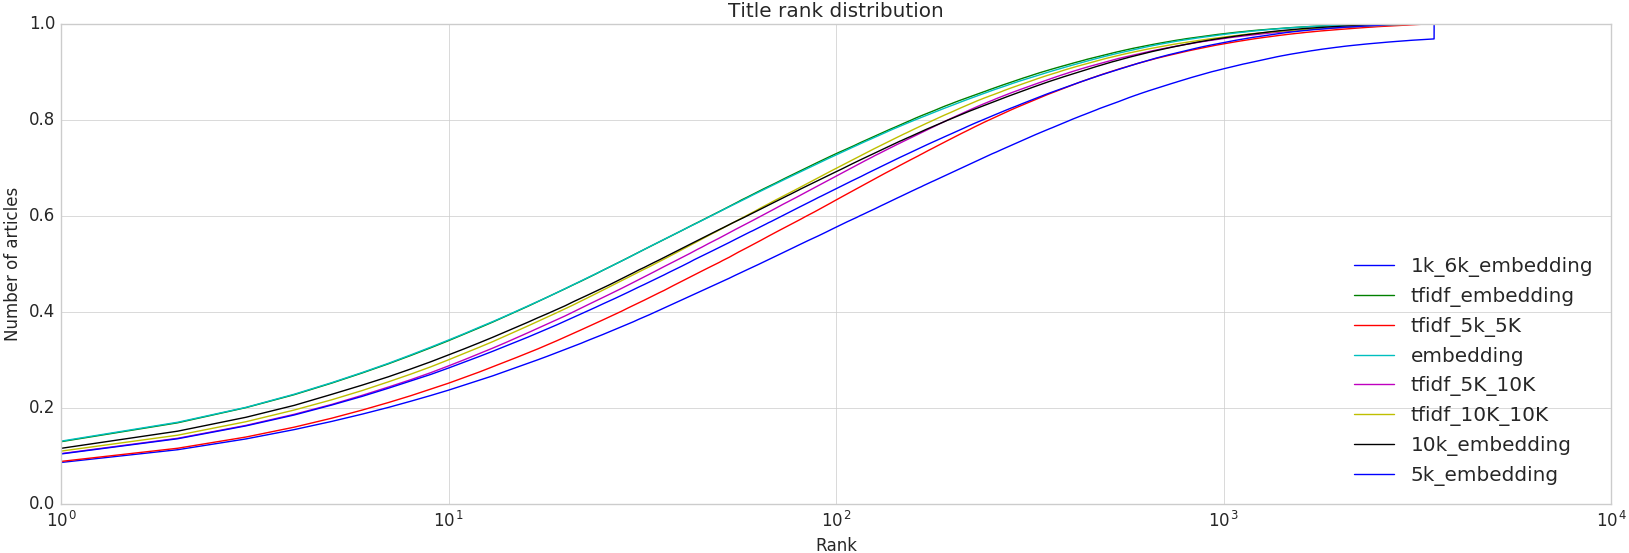
\includegraphics[width=6.5in]{Plots/Title_rank_distribution}\\
\vspace{0.2in}\\
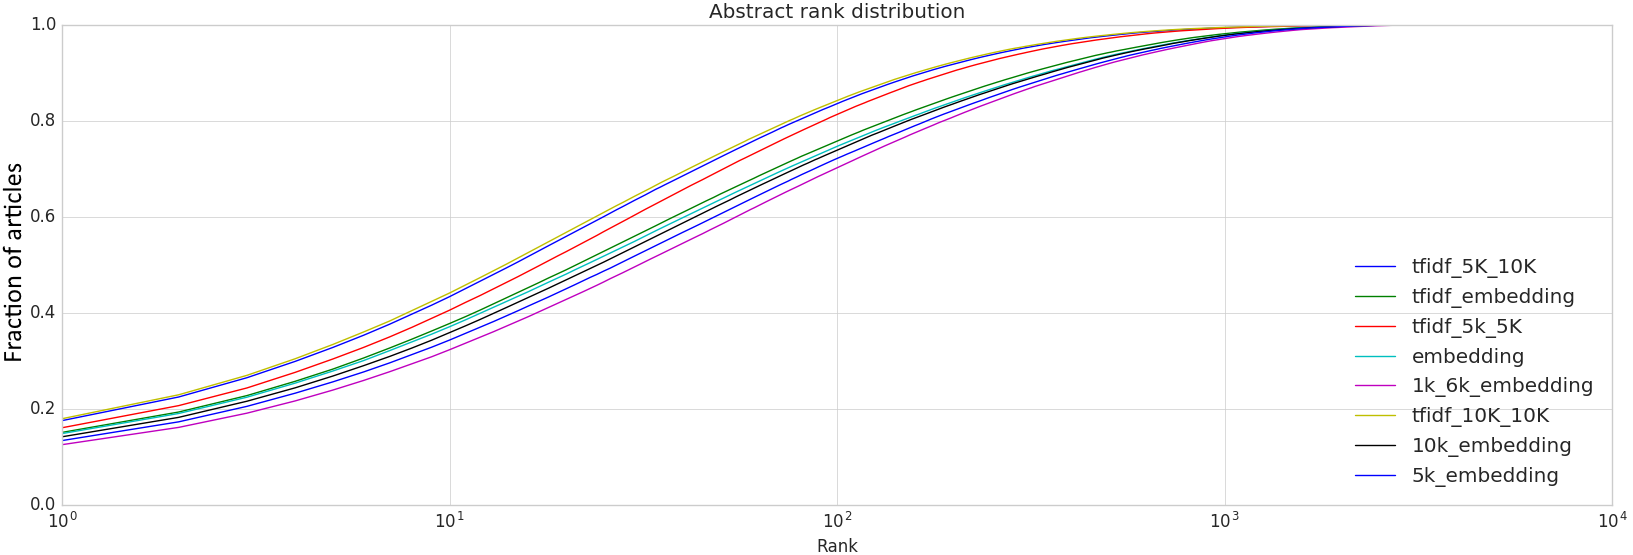
\includegraphics[width=6.5in]{Plots/Abstract_rank_distribution}\\
\clearpage
\subheader{F1-Score}
The graphs XXX and XXX show the F1 score for the title and abstract respectively. These scores are the average journals scores for each set, indicating the quality of the sets for absolute hits (top-1).\\
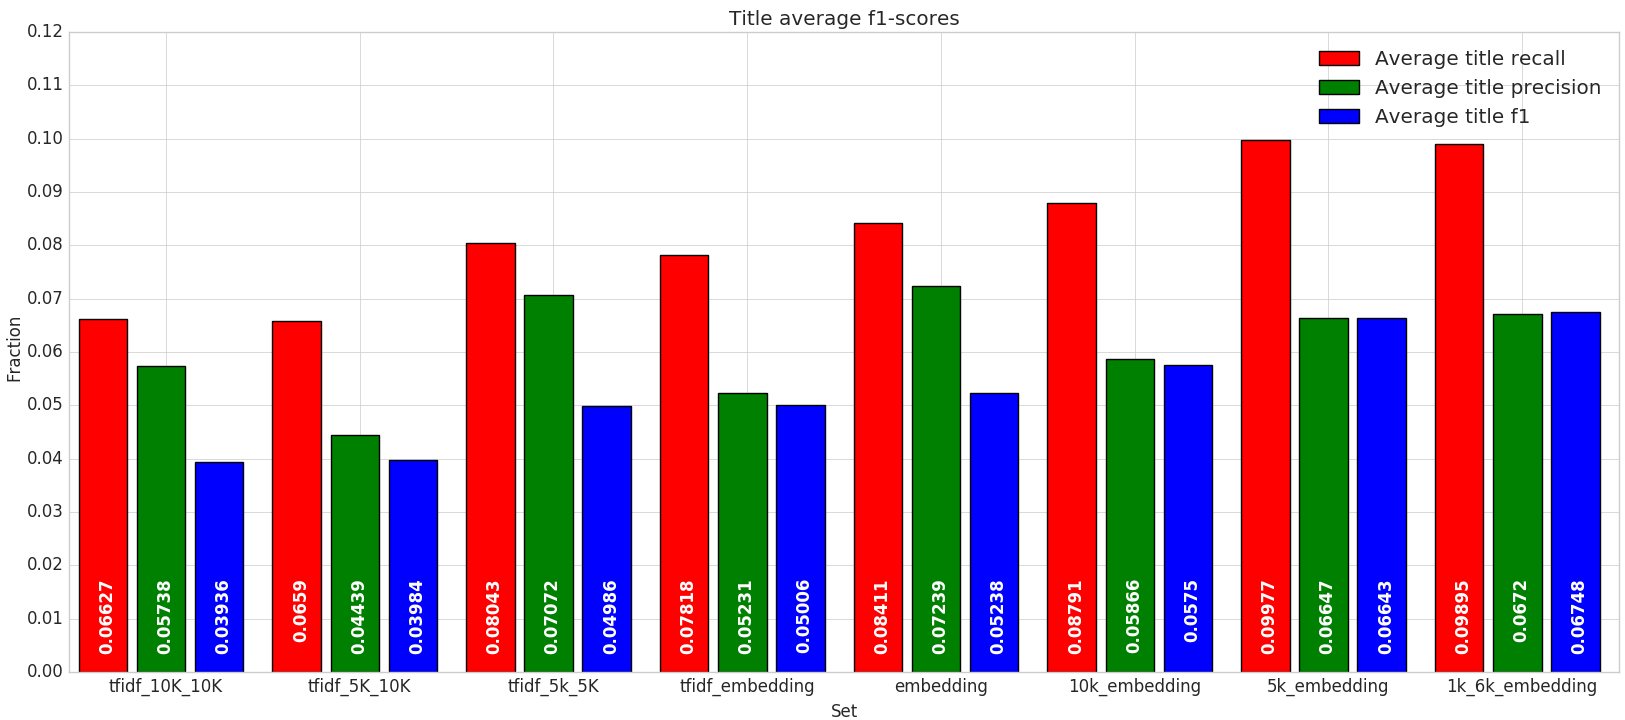
\includegraphics[width=6.5in]{Plots/Title_avg_f1}\\
\vspace{0.2in}\\
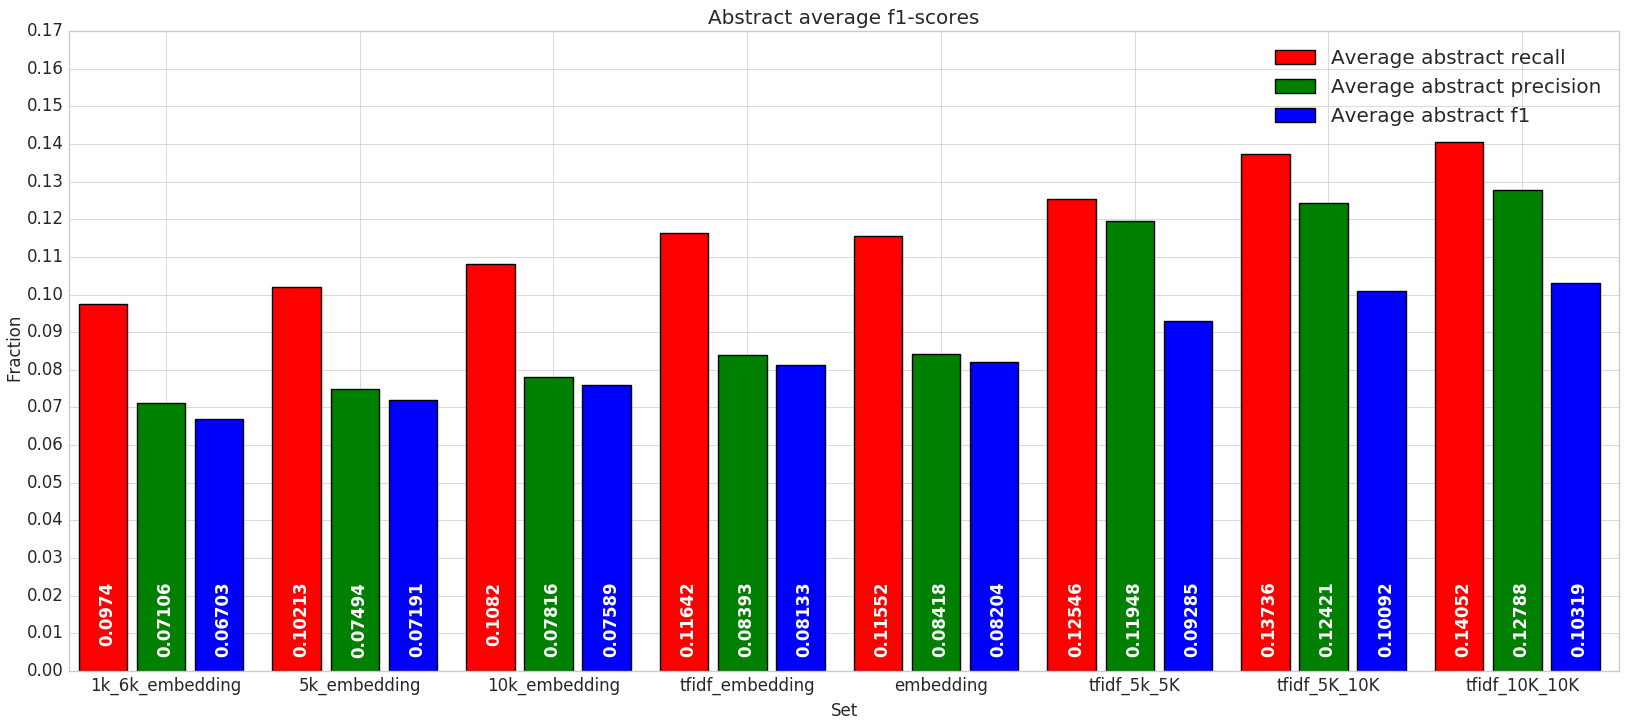
\includegraphics[width=6.5in]{Plots/Abstract_avg_f1}\\
\clearpage
\subheader{Memory usage}
XXX shows the total memory usage of each \textit{Validation set}, indicating their costs in memory storage \& RAM.\\
\begin{tabular}{|l|l|}
\hline
Set & Size in GB\\
\hline
tfidf 5k 5K & $9.82$ \\
\hline
tfidf 5K 10K & $11.47$ \\
\hline
\textbf{tfidf 10K 10K} &\textbf{11.61}\\
\hline
embedding & $3.13$ \\
\hline
5k embedding & $3.13$ \\
\hline
10k embedding & $3.13$ \\
\hline
\textbf{tfidf embedding} & \textbf{3.13} \\
\hline
1k 6k embedding & $3.06$ \\
\hline
\end{tabular}
\\

\end{document}